\section{Orientações para execução}
\subsection{Utilizando um arquivo}
Basta trocar o caminho do arquivo onde seu grafo está armazenado. O \textit{path} deve apontar para um arquivo no formato \textit{.csv} contendo duas colunas de nome \textbf{``Vi"} e \textbf{``Vj"}. Caso isso seja problemático, uma alternativa é ignorar o cabeçalho no decode do arquivo \textit{.csv}. 

\begin{table}[h!]
	\centering
	\begin{tabular}{c| cc}
		\hline
		  & Vi & Vj \\
		  \hline
		1 & A  & B \\
		2 & C  & A \\
		3 & C  & B \\
		... & ... & ... \\
		\hline
	\end{tabular}
	\caption{Formato do arquivo}
\end{table}

\subsection{Introduzindo vértices e arestas no código}
É um processo trabalhoso mas a margem para erro é virtualmente inexistente. 

\section{Entradas e testes}
\subsection{Entradas e resultados´}
\begin{figure}[h!]
	\centering
	
	\subfigure[Prática]{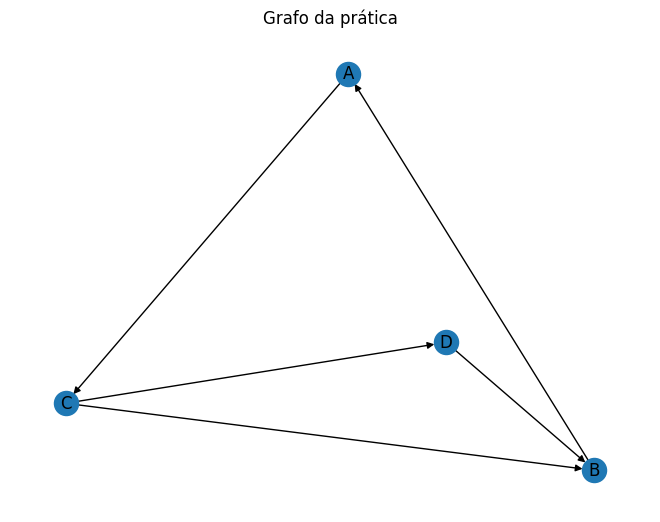
\includegraphics[width=3cm]{exercicio}}
	\subfigure[Aula]{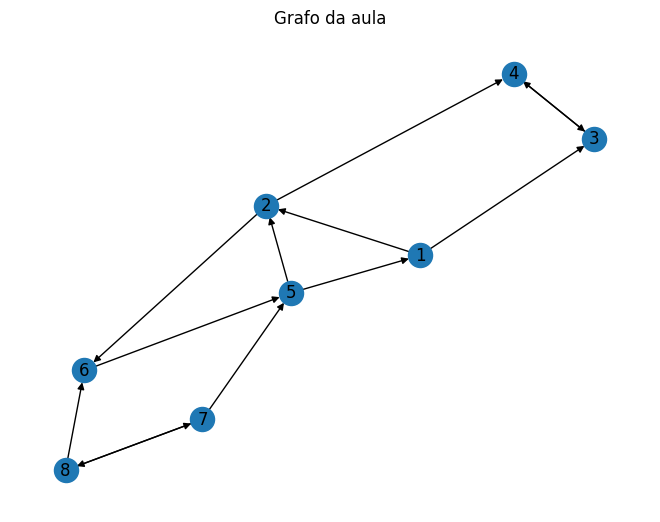
\includegraphics[width=3cm]{exercicio_aula}}
	
	\caption{Entradas}
	\label{fig:exercicio}
\end{figure}


\begin{figure}[h!]
	\centering
	
	\subfigure[Prática]{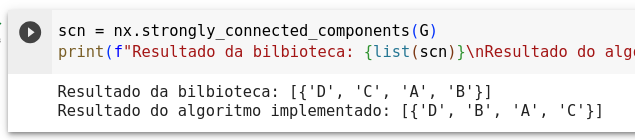
\includegraphics[height=1.5cm]{resultado}}
	\subfigure[Aula]{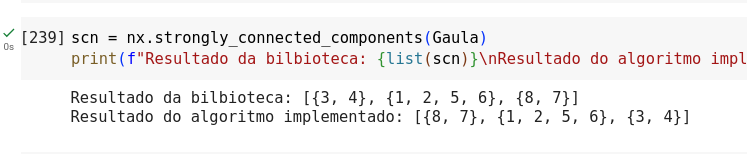
\includegraphics[height=1.5cm]{resultado_aula}}
	
	\caption{Resultados obtidos}
	\label{fig:resultado}
\end{figure}

Como podemos observar na figura \ref{fig:resultado}, os resultados obtidos estão em linha com os dados oferecidos pela biblioteca e pela resposta obtida em aula. 


\newpage


\section{Código}
O código encontra-se disponível no seguinte repositório: 
\href{https://github.com/RodrigoZonzin/grafos}{https://github.com/RodrigoZonzin/grafos}. Também está no portal.